%!TeX root = 1-screening
\documentclass[main.tex]{subfiles}

\begin{document}

\chapter{High-throughput computational screening of nanoporous materials}
\vspace*{-1\baselineskip}


\section{Materials screening toolkit}

\subsection{Nanoporous materials}

\subsubsection{Different classes of nanoporous materials}

Nanoporous materials are iupac?

definition of porosity/void fraction of surface area 

\textbf{crystalline}

Zeolite

Metal--organic frameworks (MOFs)

Covalent organic frameworks (COFs)

Porous polymer networks

\textbf{amorphous}

activated carbon 

transforming crystalline mat into amorphous one

\subsubsection{Nanoporous material databases}

\todo{Ren2021}

In the past decade, large-scale computational screening studies have become an important part of the materials science innovation pipeline,\cite{Hautier_2019, Cole_2020} trying to move beyond the serendipitous model of materials discovery.\cite{Ludwig_2019, Stein_2019} High-throughput computational discovery techniques are used in the generation of novel hypothetical structures for screening,\cite{Wilmer_2012, Boyd_2016} as well as in trying to explore more in depth and more systematically the materials whose structure has already been published, in order to map their physical and chemical properties.\cite{GomezGualdron_2014,Moliner_2019,SalcedoPerez_2019} While the idea of large-scale exploration of materials is not new, and such databases --- whether experimental or computational in the source of their data --- have been around for several decades now,\cite{PDB_1971, Grazulis_2009, Groom_2016} this field has recently seen a rapid expansion enabled by several factors. 

The first factor is the growth of public, open databases of materials structures (and sometimes properties).\cite{Coudert_2019} To give only one example, projects like the Materials Genome Initiative have~\cite{dePablo_2014, dePablo_2019} integrated theory, computation, synthesis, and characterization that led to the generation of vast materials datasets.\cite{Jain_2013, Jain_2016} Secondly, advances in the methods for construction of hypothetical structures for complex supramolecular assemblies have led to the creation of large-scale databases of hypothetical structures.\cite{Foster_2004, Wilmer_2013,Boyd_2016} Thirdly, text and data mining are allowing to augment databases with content previously thought not being machine-readable and indexable, for example by identifying unreported properties of materials in older scientific papers.\cite{Tshitoyan_2019, Court_2020} Finally, the use of artificial intelligence techniques, such as statistical learning,\cite{Butler_2018} can enable in some cases by several orders of magnitude the scale of databases that can be screened.\cite{Kim_2017, Borboudakis_2017, Chibani_2020}

Focusing more on the larger process of digital materials discovery, and the role of large databases in materials research,\cite{Zhou_2019} Boyd et al.\cite{Boyd_2017} provide a broad review of the computational developments involved in the nanoporous materials genome research effort. They show that numerous high-throughput screening studies have been targeted specifically at the question of gas phase separation, with a range of different adsorbate molecules going from noble gases, small molecules (both apolar and polar), to short alkanes and aromatics. Both Adil et al.\cite{Adil_2017} and Sturluson et al.\cite{Sturluson_2019} provide general reviews on the modelling in MOFs for gas separation and storage, and structure/separation relationships in MOFs for gas separation, featuring specific sections to the still open problem of Xe/Kr separation.

Chung et al.\ proposed a new Computation-Ready, Experimental MOF database (CoRE MOF 2019) containing over 14,000 cleaned structures.\cite{Chung_2019} The structures originated from the Cambridge Structural Database and Web of Science search. These structures went through a curation process: (i) by removing coordinates with low partial occupancies, (ii) by converting the structure to P1 symmetry, (iii) by removing free solvents (i.e., free solvent removed FSR), (iv) also removing bound solvent molecules (i.e., all solvent removed ASR), then (v) by restoring semi-automatically some disordered structures using a crystal generator. After this process, the structures are said to be ``clean''.

In this study, we used the 12,020 structures of the CoRE MOF 2019-ASR (all solvent removed) database that are publicly available. Then, we extracted the non-disordered structures and the structures with a cell volume smaller than \SI{20}{\nano\meter\cubed} (to limit the overall calculation time). This resulted in a total of 9,668 remaining structures included in our systematic simulations to compare their selectivity and other thermodynamic quantities such as enthalpy and entropy at different pressures and compositions.

\todo{Below: Ren2022}

Before building any screening strategy or performing any computational screening, one needs to generate a set of files describing the atomic structure of the materials. Nanoporous materials can have different degrees of crystallinity from perfectly crystalline to completely amorphous. Most of the computational work is focused on crystalline structures, since the atoms are well-described within a periodic framework, which enables faster simulations. The presence of defects are also usually neglected, which could explain some discrepancies between simulations and experiments. And amorphous materials are described by thousands of atomic positions in order to grasp their intrinsic non-periodicity.\cite{Thyagarajan_2020} One can distinguish roughly four main classes of crystalline nanoporous materials: the inorganic zeolites (e.g.\ aluminosilicates, aluminophosphates), the porous polymer networks, the covalent organic frameworks (COFs) and the metal--organic frameworks (containing the zeolitic imidazolate frameworks i.e.\ ZIFs and others). This diversity of nanoporous materials offer a wide range of potential candidates for any targeted applications.

The International Zeolite Association (IZA) gave a standardized set of 244 zeolites (in their idealized all-silica form) that can be used for screening purposes. To generate a dataset of structures, existing experimental database like the Cambridge Structural Database can be exploited. However, the raw structures determined experimentally by X-ray cannot be used directly as is. To obtain a computation-ready dataset, Chung et al.\ used algorithmic cleaning procedures to build the publicly available Computation-Ready Experimental MOF (CoRE MOF) database.\cite{Chung_2014, Chung_2019} CoRE MOF 2019 contains about 14,000 MOF structures, which is the biggest experimental database. Similar approach applied to organic frameworks led to the construction of a set of 187 COFs with disorder-free and solvent-free structures.\cite{Tong_2017,Ongari_2019}

These experiment-based databases can already be used in computational screenings to retrieve valuable information, but unknown structures that are yet to be discovered are not represented. To overcome the limits and biases of experimental synthesis, artificial ways of generating nanoporous material datasets can be used, which proved to be extremely efficient. The first \emph{in silico} generated database of about 130,000 MOFs used a recursion-based assembly (or tinkertoy-like) algorithm to combine 102 building blocks.\cite{Wilmer_2012} Martin and Haranczyk then proposed a topology-specific structure assembly algorithm that leverage the topological information of the structures.\cite{Martin_2014} Inspired by this algorithm, topology-based databases emerged a few years later with the set of 13,000 MOF structures generated using the Topologically Based Crystal Constructor (ToBaCCo) algorithm developed by Colon, G{\'{o}}mez-Gualdr{\'{o}}n and Snurr.\cite{Colon_2017}
Later, Boyd and Woo proposed another topology-based algorithm using a graph theoretical approach and generated a 300,000 structures database (BW-DB) based on 46 different network topologies.\cite{Boyd_2016}
Similar approaches are used for other classes of materials, Deem and coworkers proposed a dataset of nearly 2.6 million hypothetical zeolite structures.\cite{Earl_2006,Deem_2009,Pophale_2011}
However, one could wonder if these hypothetical structures are synthesizable and can remain stable under operational conditions (e.g.\ thermal, mechanical, radioactive constraints). To discuss their synthetic likelihood, Anderson and G{\'{o}}mez-Gualdr{\'{o}}n computed the free energies of 8,500 hypothetical structures and compared them to experimentally observed MOF structures.\cite{Anderson_2020}
Later, Nandy et al.\ performed a meta-analysis of thousands of articles associated to the CoRE MOF 2019 database to extract their experimental solvent-removal stability and thermal decomposition temperature.\cite{Nandy_2021} These data are then leveraged in the training of multiple ML models to predict stability properties. These predictions can be very useful to gauge the relative stability of each materials and to only consider stable structures. Other types of materials have been explored, Turcani et al.\ published 60,000 organic cage structures and used machine learning to predict their stability based on the shape persistence metric.\cite{Turcani_2018}

The Materials Genome Initiative, a 100 million dollar effort from the White House that aims to ``discover, develop, and deploy new materials twice as fast'', led to the creation of the ``Materials Project'', a centralized database containing all the above mentioned structures.\cite{kalil2011national,Matgenome,Jain_2013}
The fast development of this nanoporous materials genome motivated Boyd et al.\ to write a comprehensive review on all the initiatives on generating new data for computational analysis.\cite{Boyd_2017}

Yet, the sole increase in size of the databases is not enough. One needs to add diversity to have more general knowledge on the maximum performance and the explanatory features of such performance. Moreover, the diversity of structures ensure the quality of the predicted best materials for a given application.
To qualitatively or quantitatively assess the diversity of a database, inventive methodologies have been developed.
For instance, Martin, Smit and Haranczyk proposed a Voronoi hologram representation as a way of measuring similarities between structures to generate geometrically diverse subsets of a database.\cite{Martin_2011}
Moosavi et al.\ made a comparative study of the diversity of three well-known databases CoRE MOF 2019,\cite{Chung_2019} BW-DB\cite{Boyd_2016} and ToBaCCo\cite{Gomez_Gualdron_2016, Colon_2017}  using geometrical and chemical descriptors to design a theoretical strategy for generating the most diverse set of materials.\cite{Moosavi_2020}
Another approach consists in searching for similarities instead of differences in the materials by studying topological patterns in the data.\cite{Lee_2017}
These investigations on the data structures give a solid ground to develop novel materials by objectively defining similarity, diversity and novelty. From the analysis gathered so far, one would need to radically change the approach by proposing materials with new chemistry, topology or mechanism (e.g.\ flexibility) in order to significantly improve the diversity of the current databases.

\subsection{Screening methodologies}

In its early stage, computational screening has been used on small series of nanoporous materials to generate specific knowledge on some subclasses of materials. These small-scale screenings combined with experiments helped faster identification of good performing candidates, but they failed to establish general rules of design or to explore the unknown. Larger-scale screenings overcame these limitations by trying to exhaustively cover the whole spectrum of nanoporous materials.

With the development of a nanoporous materials genome, several articles proposed methods to screen thousands of structures. Other challenges arose, such as the design of more efficient methods than the brute force screening or the analysis of big data. Two research groups in Northwestern University led by R. Snurr and J. Hupp began to address those questions, they used a ``funnel-like'' approach to efficiently screen about 130,000 hypothetical MOF structures.\cite{Wilmer_2012} To do so, they performed a first screening involving fewer steps of simulation on the whole dataset, then they extracted a subset of top performing structures to perform a second round with more simulation steps. This procedure is repeated until a few materials are selected by a final round of simulations with reasonable accuracy.
Similar ``funnel-like'' procedures have then been used in other field of applications as described in the Figure~\ref{fgr:screening}. This type of screening saves precious computation time by balancing the complexity of the calculation with the amount of data to be screened. The most demanding simulations or experiments are only applied to the few most promising structures.
This method can rather efficiently identify top candidates, but it can't draw quantitative structure-property relationships (QSPR), beside facing scalability issues above a critical dataset size.

To overcome these new challenges, people are looking increasingly towards transferable models trained by a machine learning (ML) algorithm on a diverse and size-limited sub-sample. Ideally, such a model is transferable to potentially millions of structures and can provide valuable QSPR. For instance, Fernandez et al.\cite{Fernandez_2013} used multiple linear regression analysis, decision tree regression, and nonlinear support-vector
machine models to extract QSPR and establish rules of designing well-performing MOFs for methane storage, while identifying promising structures. In this first work they only used geometrical descriptors to describe methane storage,\cite{Fernandez_2013} but realizing the importance of chemical descriptors, they proposed the atomic property weighted radial distribution function as a powerful descriptor to predict CO$_2$ uptakes.\cite{Fernandez_2013_rdf}
More importantly, they proved that ML can be used as a pre-screening tool to avoid running time-costly simulations by correctly identifying around \SI{95}{\percent} of the top 1000 best performing materials. Recently, the same group used similar techniques to predict CO$_2$ working capacity as well as CO$_2$/H$_2$ selectivity in MOFs for pre-combustion carbon capture.\cite{Dureckova_2019}

\begin{figure*}[t]
    \centering
      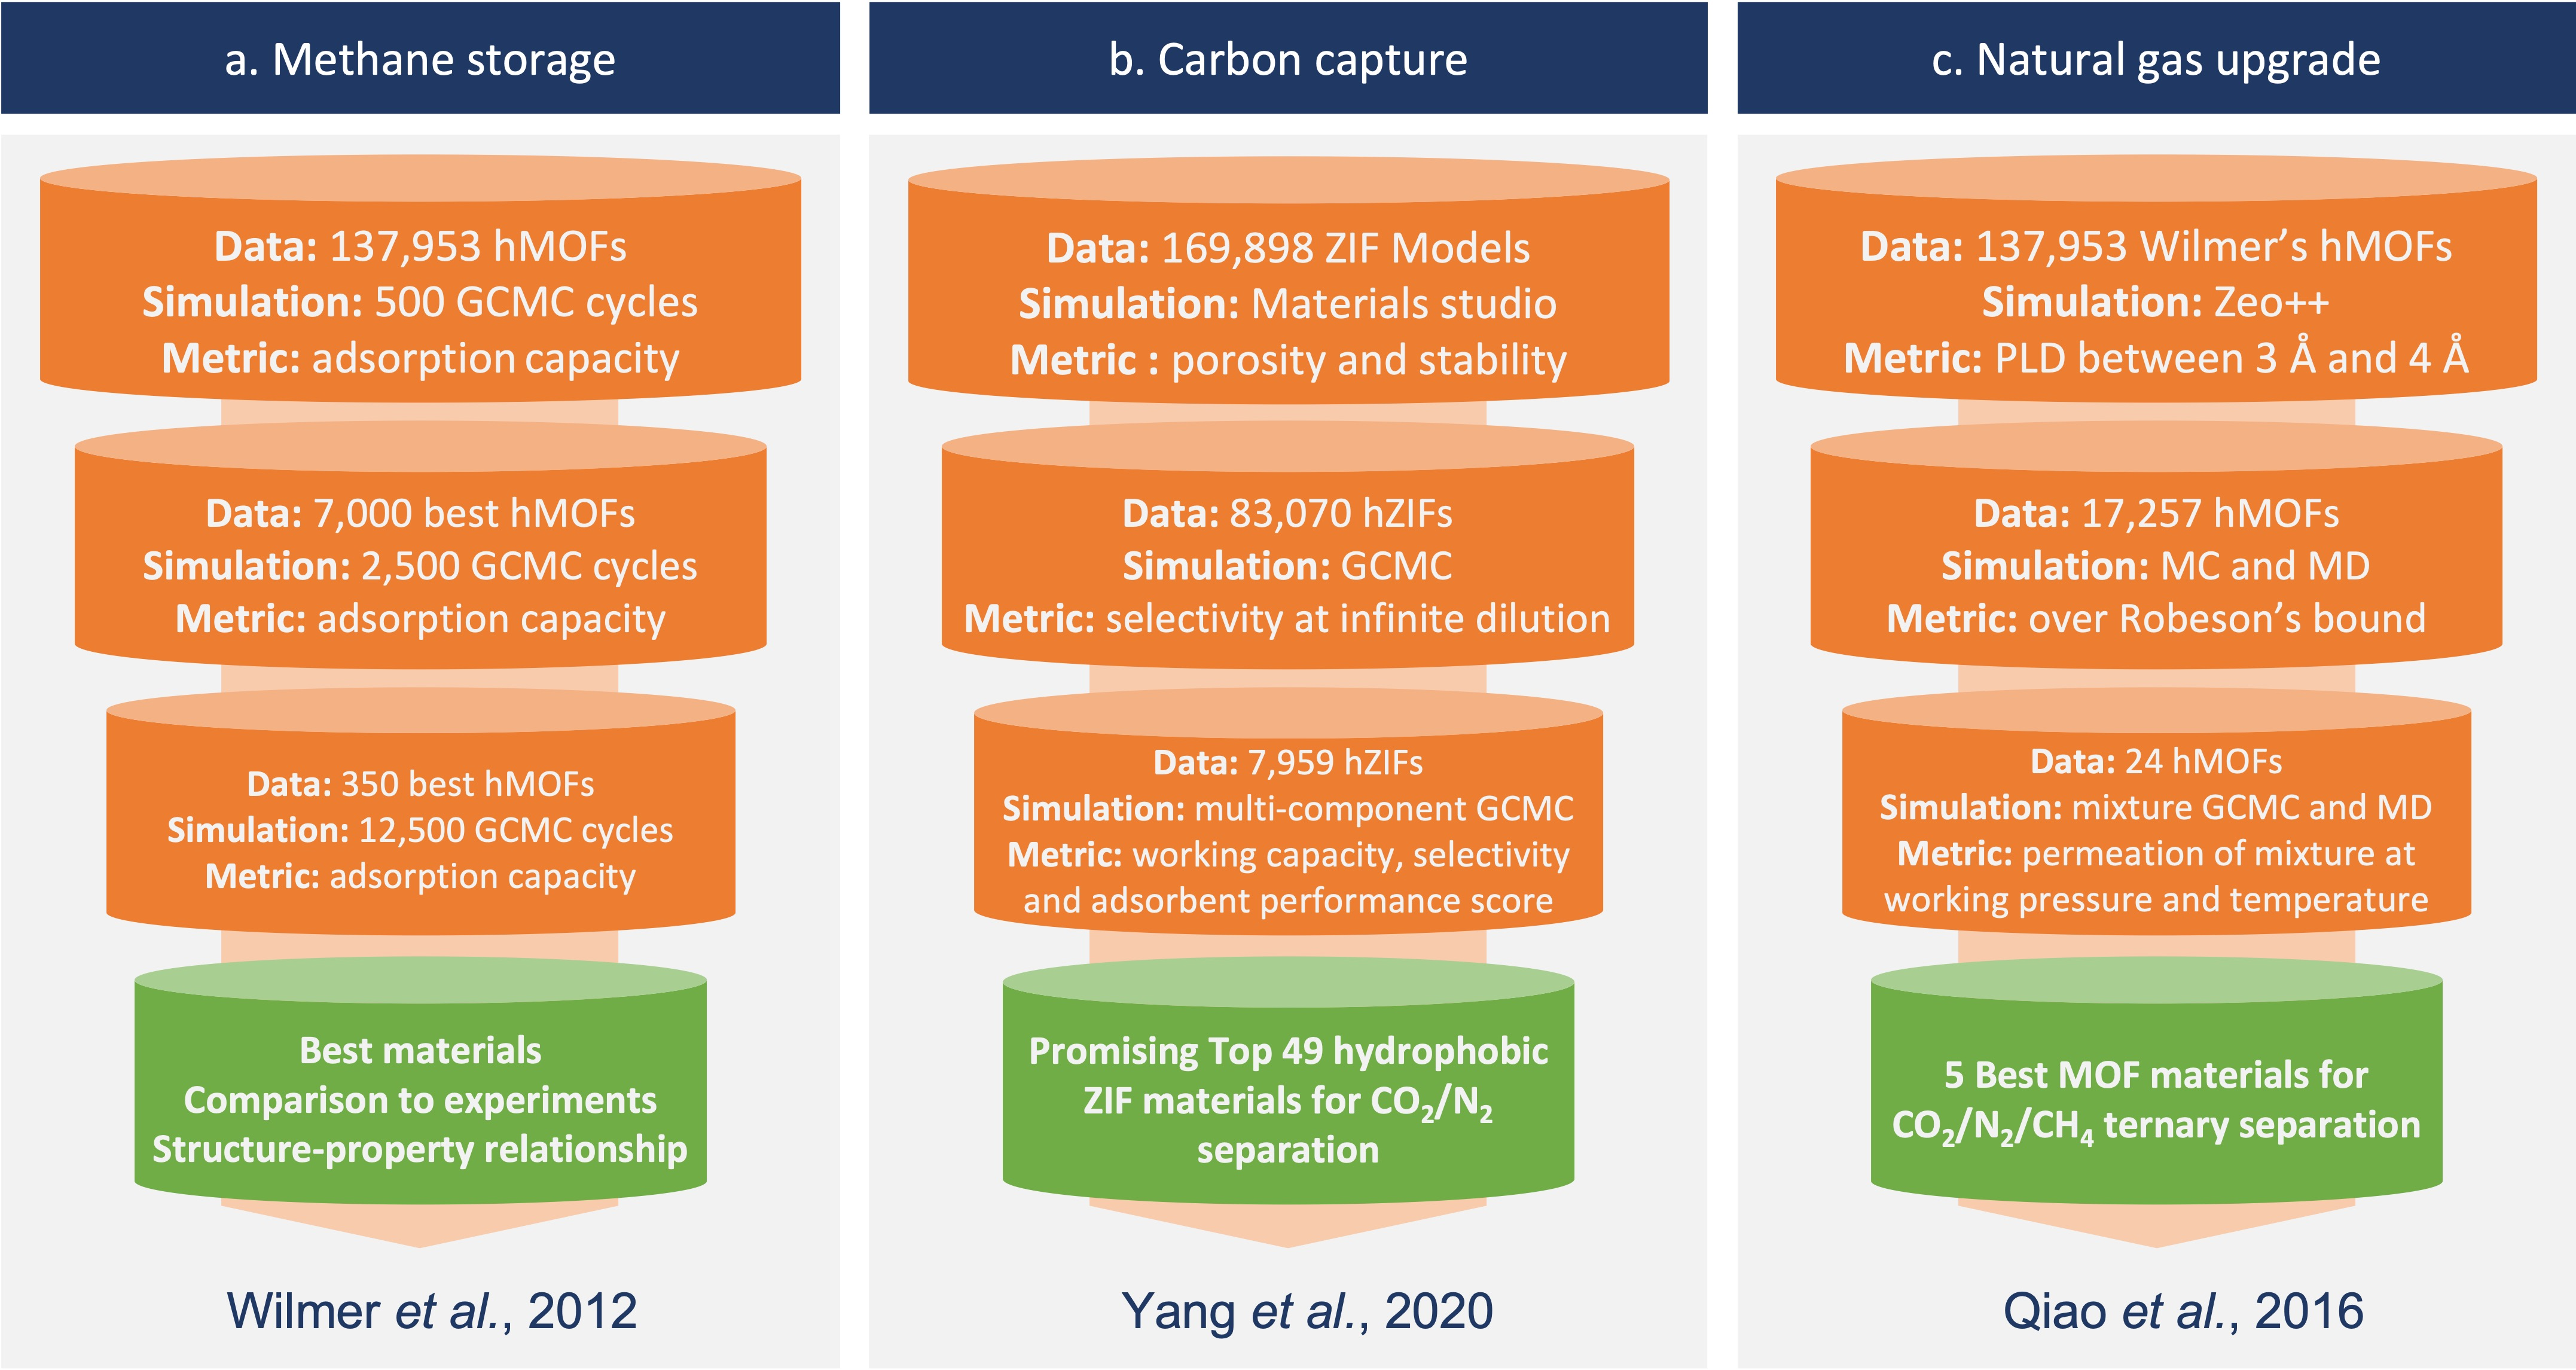
\includegraphics[width=\textwidth]{figures/1-screening/Screening_procedures.jpg}
      \caption{Simplified representation of typical funnel-type screening procedures, exemplified on three different applications from the published literature. (a) Wilmer et al.\cite{Wilmer_2012} used a series of bi-component Grand Canonical Monte Carlo (GCMC) calculations at different levels of complexity to screen a large dataset of hypothetical MOFs for methane storage application. (b) Yang et al.\cite{Yang_2020} used simulations at infinite dilution to pre-screen the dataset before using computationally demanding simulations and multiple metrics to find the most promising ZIFs for carbon capture. (c) In Qiao et al.\cite{Qiao_2016}, transport properties were screened along standard adsorption properties to find the best materials for the targeted CO$_2$/N$_2$/CH$_4$ ternary separation; similarly, cheaper calculations at infinite dilution were carried out in a first step, before using more expensive calculations at working pressure and temperature.}\label{fgr:screening}
    \end{figure*}

\subsection{Machine learning assisted screening}

\todo{Simon sumup}

In 2015, Simon et al.\cite{Simon_2015} analyzed the Nanoporous Materials Genome,\cite{Simon_2015_EES, Boyd_2017} a database of about 670,000 experimental and hypothetical porous material structures, including MOFs, zeolites, PPNs, ZIFs, and COFs, for candidate adsorbents for xenon/krypton separations. It is possibly the largest-scale study performed in this area, both by the sheer number of frameworks involved and by the diversity of their nature. Because such a set is too big for brute-force screening with GCMC simulations, they proposed a multiscale modelling strategy combining machine learning algorithms (trained on a diverse subset of 15,000 materials) with molecular simulations (used both to generate the ML training data, and to refine the separation properties for the top performers obtained by the ML predictor). Without going into details (see Fig.~\ref{fgr:Simon} for more details), the ML model they trained was mainly based on geometric structural descriptors, with the addition of a single energy-based descriptor: the Voronoi energy\ (i.e.\ the average energy\ of a xenon atom at the accessible nodes in the Voronoi partition of space). In addition to identifying and describing some top performing materials, the authors also analyzed the correlations between high Xe/Kr selectivity and the geometric properties of the frameworks, in order to ``rationalize the strong link between pore size and selectivity''. In particular, by developing theoretical pore models of spherical and cylindrical geometries, they could highlight the general geometrical trends observed, but also the fact that there is a wide diversity of performance beyond the geometrical features of the frameworks.

\begin{figure*}[t]
    \centering
    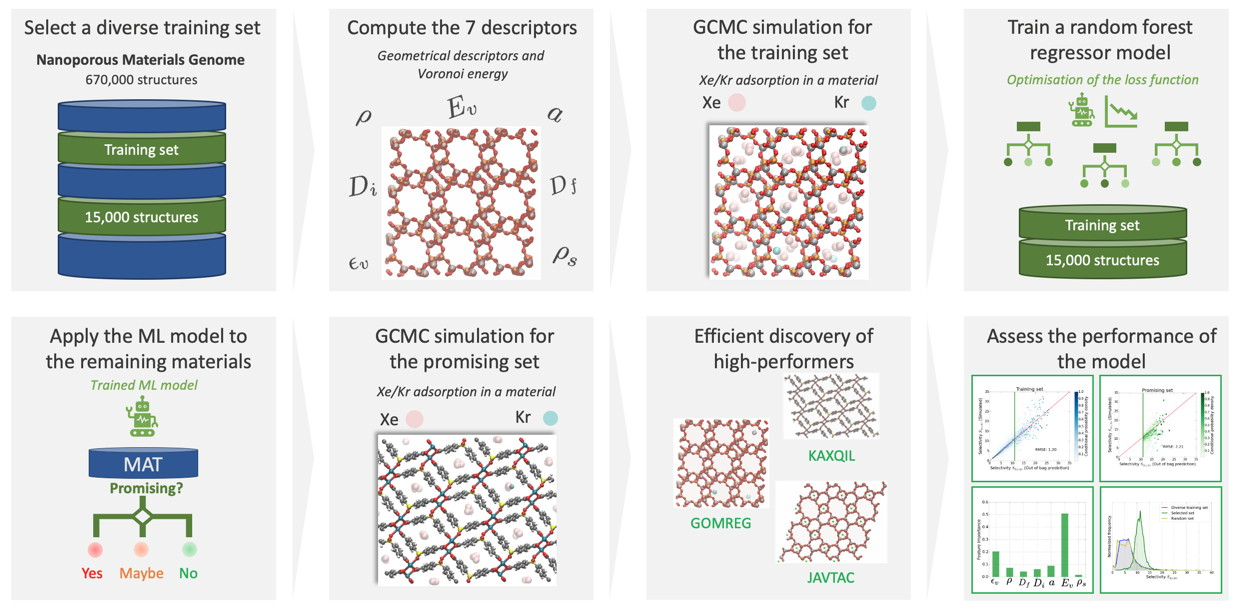
\includegraphics[width=0.99\textwidth]{figures/1-screening/Simon.jpg}
    \caption{\ Schematic representation of large-scale screening of nanoporous materials for Xe/Kr adsorption-based separation by Simon et al.,\cite{Simon_2015} based on a combination of Grand Canonical Monte Carlo simulations and machine learning algorithm (Random Forest Regressor). The main goal of this screening is to find high-performing materials in a large dataset of both experimental and hypothetical materials. 
    Adapted with permission from Ref.~\citenum{Simon_2015}. Copyright 2015 American Chemical Society.
    }\label{fgr:Simon}
\end{figure*}

\section{An overview of the literature}

\subsection{Thermodynamic adsorption properties}

\subsubsection{Gas storage}



\subsubsection{Gas separation}

\subsection{Transport adsorption properties}

\subsubsection{Kinetic properties}

Used in breakthrough simulation

\subsubsection{Membrane materials}

\subsection{Non-adsorption properties}

\subsubsection{Catalytic activity}

\subsubsection{Mechanical properties}

\subsubsection{Thermal properties}

\section{Consequences for xenon/krypton separation}

\subsection{Status quo}

\subsubsection{What is done in Xe/Kr separation}

\subsubsection{What can be learned in the other fields}

\subsection{Future perspectives}

Main improvement points

\subsubsection{Faster energy sampling}
Integration in ml
\subsubsection{Faster diffusion estimation}



\subsubsection{Flexibility OMS}

\OnlyInSubfile{\printglobalbibliography}

\end{document}
